 \documentclass[10pt]{article}
 \usepackage[margin=1.2in,a4paper]{geometry}
 \usepackage[T1]{fontenc}
 \usepackage{textcomp}
 \usepackage{ragged2e}
 \usepackage{booktabs}
 \usepackage{epltxfn} %expex footnotes
 \usepackage{bold-extra}
 \usepackage{fancyhdr}
 \usepackage{fontspec,xltxtra,xunicode}
 \usepackage[labelsep=period,font=small,labelfont=bf,small]{caption}
 \defaultfontfeatures{Mapping=tex-text}
 \setmainfont{Cambria}
 \newcommand{\HRule}{\rule{\linewidth}{0.5mm}}
 %\setromanfont[Mapping=tex-text]{Hoefler Text}
 %\setsansfont[Scale=MatchLowercase,Mapping=tex-text]{Gill Sans}
 %\setmonofont[Scale=MatchLowercase]{Andale Mono}
 
 
 \usepackage{Sanremo,lettrine}
 \renewcommand\LettrineFontHook{\Sanremofamily}
 
 % \usepackage[margin=.7in,nohead,right=1.5in]{geometry}
 \def\singlesidestandardsetup{
 	%\textwidth 6in
 	%\oddsidemargin 0in
 	%\evensidemargin 0in
 	%\topmargin -.5in
 	
 	%\textheight 9.5in
 	%\columnwidth \textwidth
 	\parindent 1em
 	%\parskip 8pt
 	\pagenumbering{roman}
 	\parindent 1em
 	\parskip 10pt
 	
 }
 \usepackage{marginnote}
 \xdef\marginnotetextwidth{\the\textwidth}
 
 \usepackage{wrapfig}
 %\newcommand{\longsquiggly}{\xymatrix@C=1.915em{{}\ar@{~>}[r]&{}}}
 
 \fancypagestyle{plain}{%
 	\fancyhf{} % clear all header and footer fields
 	\fancyfoot[C]{\sffamily\fontsize{9pt}{9pt}\selectfont\thepage} % except the center
 	\renewcommand{\headrulewidth}{0pt}
 	\renewcommand{\footrulewidth}{0pt}}
 \pagestyle{plain}
 
 
 \newcommand{\mcom}[1]
 {\marginpar{\raggedleft\raggedright\hspace{0pt}\linespread{0.9}\footnotesize{#1}}}
 \newcommand{\cb}[1]
 {\marginpar{\color{orange}\raggedleft\raggedright\hspace{0pt}\linespread{0.8}\footnotesize{#1}}}
 \newcommand{\hk}[1]
 {\marginpar{\color{purple}\raggedleft\raggedright\hspace{0pt}\linespread{0.8}\footnotesize{#1}}}
 
 \newcommand{\mmp}[1]
 {\marginpar{\color{green}\raggedleft\raggedright\hspace{0pt}\linespread{0.8}\footnotesize{#1}}}
 
 \newcommand{\note}[1]{{ }\mcom{Note}\textbf{#1}}
 
 \newcommand{\glem}[1]
 {\MakeUppercase{\scriptsize{\textbf{#1}}}}
 
 
 %%%%cancel margin notes
 \renewcommand{\mcom}[1]{}
 \renewcommand{\mmp}[1]{}
 \renewcommand{\cb}[1]{}
 \renewcommand{\hk}[1]{}
 
 \newcommand{\specialcell}[2][c]{%
 	\begin{tabular}[#1]{@{}c@{}}#2\end{tabular}}
 
 \makeatletter
 \def\@xfootnote[#1]{%
 	\protected@xdef\@thefnmark{#1}%
 	\@footnotemark\@footnotetext}
 \makeatother
 
 
 \newcommand{\xmark}{\ding{55}}
 
 
 
 \author{Josh}
 \date{\today}
 
 \usepackage{subfigure}
 \usepackage{amsthm}
 \usepackage[normalem]{ulem}
 \usepackage{amssymb}
 \usepackage{multirow}
 \usepackage{mathrsfs}
 \usepackage{pifont}
 \usepackage{mathtools}
 \usepackage{tikz}
 \usepackage{qtree}
 \usepackage{tikz-qtree}
 %\usepackage{tipa}
 \usetikzlibrary{decorations.pathreplacing}
 \usepackage{textcomp}
 \usepackage[normalem]{ulem}
 \usepackage{url}
 \usepackage[all]{xy}
 \usepackage{multicol}
 \usepackage{hanging}
 \usepackage{booktabs}
 \usepackage{setspace}
 \usetikzlibrary{shapes,backgrounds}
 \usepackage{geometry}
 
 
 
 \newtheorem{definition}{Definition}
 \newtheorem{theorem}{Theorem}
 
 
 \usepackage{enumerate}
 \usepackage{enumitem}
 %\usepackage{gb4e} \let\eachwordone=\sl
 \usepackage{expex}
 
 
 
 %\newcommand{\denote}[1]{\mbox{$[\![\mbox{#1}]\!]$}}
 \newcommand{\concat}{\mbox{$^\frown$}}
 \newcommand{\ph}{\varphi}
 \newcommand{\vsep}{\vspace{8pt}}
 \newcommand{\linesep}{\rule{6.5in}{.5pt}}
 \def\attop#1{\leavevmode\vtop{\strut\vskip-\baselineskip\vbox{#1}}}
 \newcommand{\denote}[1]{\mbox{$[\![\mbox{#1}]\!]$}}
 \newcommand{\exref}[1]{~(\ref{#1})}
 
 \newcounter{nextsec}
 \newcommand\nextsection{%
 	\setcounter{nextsec}{\thesection}%
 	\stepcounter{nextsec}%
 	\thenextsec%
 }
 \newcommand\nextsubsection{%
 	\setcounter{nextsec}{\expandafter\parsesub\thesubsection\relax}%
 	\stepcounter{nextsec}%
 	\thesection.\thenextsec%
 }
 \def\parsesub#1.#2\relax{#2}
 \def\parsesubsub#1.#2.#3\relax{#3}
 %\input{setup}
 
 %\singlesidestandardsetup
 
 %\parindent 1em
 
 %\input{psfig-scale}
 
 
 \newcommand{\verteq}{\rotatebox{90}{$\,=$}}
 \newcommand{\equalto}[2]{\underset{\scriptstyle\overset{\mkern4mu\verteq}{#2}}{#1}}
 
 
 \newcommand{\secsep}{\hrulefill}
 \renewcommand*{\marginfont}{\small}
 \usepackage{qtree}
 \qtreecenterfalse
 
 \renewcommand{\baselinestretch}{1} %% this is the linespacing
 
 \newcommand{\la}{\langle}
 \newcommand{\ra}{\rangle}
 \newcommand{\lamda}{\lambda}
 \usepackage{framed}
\begin{document}

\Large\textbf{The intersection of temporal \& modal interpretation}

\large\textbf{A view from Arnhem Land}


\small\textit{Prospectus defense}\hfill\today

\subsection*{Kriol apprehensionality \texttt{[rop]}}

\pex\label{ssq0}\begingl
\gla main dedi imin go la det shop ailibala \textbf{bambai} imin kambek bla gugum dina bla melabat//
\glb my father 3s\textdblhyphen{}{\sc pst} go {\sc loc} the shop morning \textit{\textbf{bambai}} 3s\textdblhyphen{}{\sc pst} come.back {\sc purp} cook dinner {\sc purp} 1p{\sc.excl}//
\glft`My dad went to the shop this morning, \textbf{then} he came back to make lunch for us' \hspace*{\fill}(AJ~23022017)//
\endgl\xe

\pex\textbf{Context:} I've invited a friend around to join us for dinner. They reply:	
\a\begingl\deftagex{pres}\deftaglabel{seq}
\gla yuwai! \textbf{bambai} ai gaman jeya!//
\glb yes! \textit{\textbf{bambai}} 1s come there//
\glft `Yeah! I'll be \textbf{right} there!'//
\endgl
\a\deftaglabel{m}\begingl\deftaglabel{appr}
\gla najing, im rait! \textbf{bambai} ai gaan binijim main wek!//
\glb no 3s okay \textit{\textbf{bambai}} 1s \textsc{neg.mod} finish 1s work//
\glft`No, that's okay! (If won't, \textbf{otherwise}) I mightn't (be able to) finish my work!'\hfill(GT13072017)//\endgl\xe

\pex\textbf{Context:} A child is playing on a car and is told to stop.
\a	\begingl 	\gla gita la jeya!//
\glb get~off {\sc loc} there!//
\endgl
\a[label=\textcolor{gray}{B}]\begingl\gla \textcolor{gray}{ba~wani?}//
\glb \textcolor{gray}{why?}//
\endgl
\a[label=A]\begingl
\gla bambai yu breigim motika//
\glb \textbf{\textit{bambai}} 2s break car//
\glft `Get off of there [...why?...] In a moment you'll break the car!'\hspace*{\fill}(GT~16032017)//\endgl\xe

\subsection*{Yolŋu TMA}
\pex<wangI>\label{wangI} \textbf{Apparent insensitivity of verbal morphology to tense distinction in Wangurri \texttt{[dhg]}}
\a\begingl
\glpreamble \textsc{Nonfuture use}//
\gla nhän \textbf{gayŋa} ŋirrima-ḻi \textbf{ŋarra}//
\glb 3s \textsc{ipfv} home-\textsc{all} go.\textbf{I}//
\glft`they went/were going home' (\textsc{pst}) \textbf{\textit{or}} `they're going home' (\textsc{pres})//
\endgl 
\a\begingl \glpreamble\textsc{Future use}//
\gla nhän \textbf{ŋarru} ŋirrima-ḻi \textbf{ŋarra}//
\glb 3s \textsc{irr} home-\textsc{all} go.\textbf{I}//
\glft`they will/should/must go home'\hfill(\texttt{[dhg]} McLellan 1992:154)//
\endgl
\xe

\pex \textbf{Cyclicity and metricality in Djambarrpuyŋu \texttt{[dhg]}}
\a\deftagex{pasts}\begingl\glpreamble\textsc{Recent past with \textbf{I}}//
\gla yo barpuru-ny ŋarra ŋaɲa nhä-\textbf{ma}-ny (*nhäŋal)//
\glb	yes, yesterday{\sc-prom} 1s 3s{\sc.acc} see-\textbf{I/*III}-{\sc prom}//
\glft`Yes, I saw him yesterday'\footnotemark//\endgl
\a\begingl\glpreamble\textsc{Today past with \textbf{III}}//
\gla ŋe gäthur ŋarra ŋanya nhä-\textbf{ŋal} goḏarr dhiyal//
\glb	yes, today 1s 3s{\sc.acc} see-\textbf{III} morning {\sc prox-loc}//
\glft`Yes, I saw him here this morning'//\endgl
\a\begingl\glpreamble\textsc{Distant past with \textbf{III}}//
\gla maarrma ga-\textbf{n} malwan-dja dhära-\textbf{n} yindi maṉḏa-ɲ//
\glb two {\sc ipfv-\textbf{III}} Hibiscus-{\sc prom} stand-\textbf{III} big 3d-{\sc prom}//
\glft`Two big Hibiscus flowers were growing there' (at some place in the speaker's youth)\hfill(Wilkinson 1991: 339)//
\endgl
\xe


\begin{figure}[h!]
\caption{Schematisation of inflectional domains (Wilkinson 1991:362)}

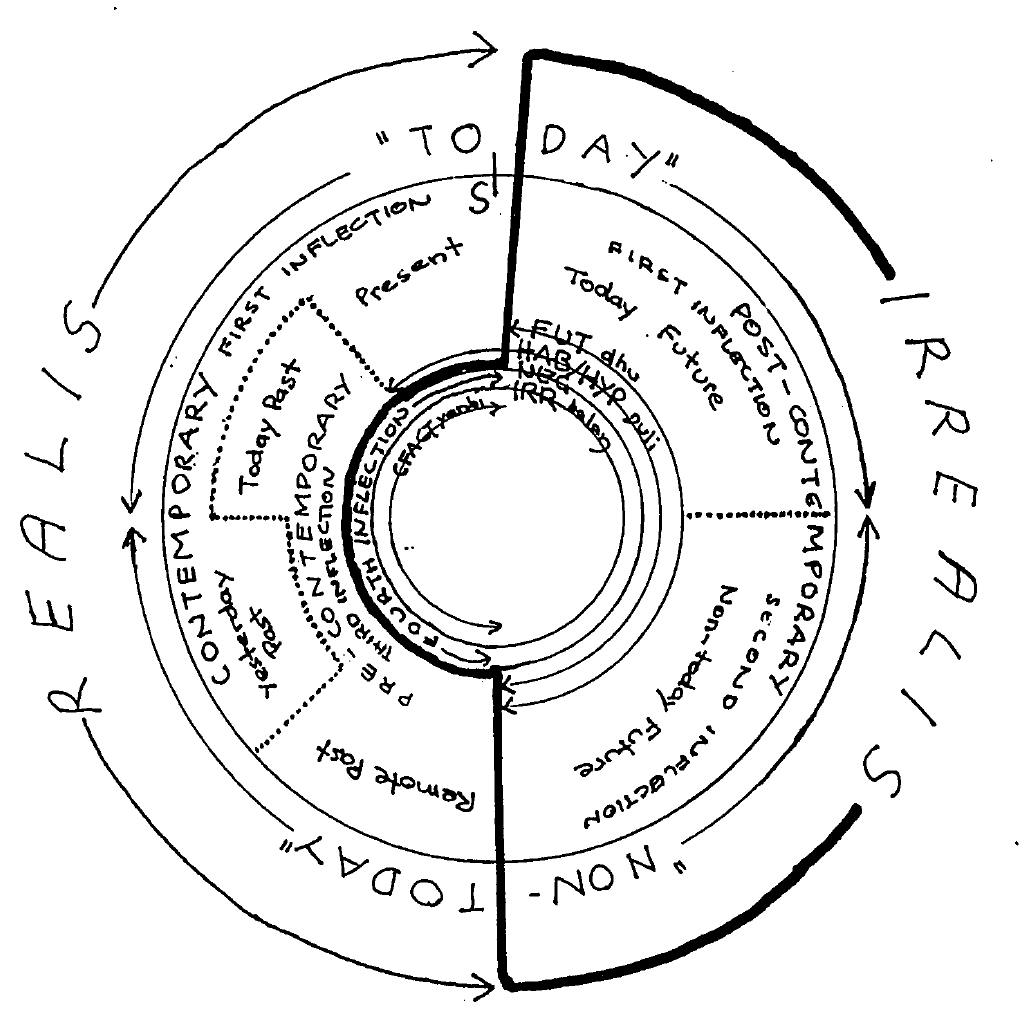
\includegraphics[scale=.7]{/Users/joshphillips/Dropbox/dissertation/prospectus/WilkinsonDiagram362.png}

\end{figure}
\end{document}